% -*- coding: utf-8 -*-

\begin{chapter}{Влияние атмосферы на океан}\label{chap:4}
% \chapter{Atmospheric Influences}
Солнце и земная атмосфера прямо и косвенно оказывают определяющее
влияние на все динамические процессы в океане. Основные внешние по
отношению к океану источники и стоки энергии: солнечный свет, испарение,
инфракрасное излучение с поверхности океана и, наконец, изменение температуры
океана под действием холодных и теплых ветров.
%% ???"sensible heating of the sea by warm or cold winds"
%% как может возникать нагрев под действием холодного ветра? сносом воды,
%% которую замещает более теплая?
Влияние ветра на циркуляцию поверхностных вод распространяется на
глубины до~$1\km$, а ветровое и приливное перемешивание
управляют глубинными океаническими течениями.
%
% The sun \index{sun}and the atmosphere drive directly or indirectly almost 
% all dynamical processes in the ocean. The dominant external sources and 
% sinks of energy are sunlight, evaporation, infrared emissions from
% the sea surface, and sensible heating of the sea by warm or cold winds.
% Winds drive the ocean's surface circulation down to depths of around
% a kilometer. Wind and tidal mixing\index{mixing!tidal}
% drive the deeper currents in the ocean.

Океан, в свою очередь, служит источником тепла, определяющим атмосферную 
циркуляцию. Отсутствие
равновесия между притоком тепла в океан и его оттоком приводит 
к возникновению в атмосфере ветров. Солнечное излучение прогревает воды 
в тропиках. Испарение с прогретой поверхности океана приводит 
к переносу тепла из океана в атмосферу вместе с водяными парами. Это тепло
высвобождается при конденсации, когда водяные пары выпадают в виде осадков.
Ветры и океанические течения переносят тепло от экватора к
полюсам, откуда оно передается в космос.%
\remark{В низких широтах Земля получает больше тепла от Солнца, чем теряет 
его путём собственного излучения, в высоких широтах~--- наоборот. 
Междуширотный обмен воздухом приводит к переносу тепла из низких широт 
в высокие и холода из высоких широт в низкие, чем сохраняется тепловое 
равновесие на всех широтах Земли. 
(Ст.\ <<Циркуляция атмосферы>>, БСЭ 
(\href{http://slovari.yandex.ru/dict/bse/article/00088/46000.htm}%
{\url{http://slovari.yandex.ru/dict/bse/article/00088/46000.htm}}))}
%
% The ocean, in turn, is the dominant source of heat that drives the 
% atmospheric circulation.\index{atmospheric circulation!driven by ocean}
% The uneven distribution of heat loss and gain by the ocean leads to winds
% in the atmosphere. Sunlight warms the tropical ocean, which evaporate,
% transferring heat in the form of water vapor to the atmosphere. The heat
% is released when the vapor condenses as rain. Winds and ocean currents
% carry heat poleward, where it is lost to space.

Поскольку атмосфера влияет на динамику океана, а океан, в свою
очередь, также влияет на атмосферную циркуляцию, мы должны
рассматривать океан и атмосферу как единую динамическую систему. В
этой главе мы затронем, в основном, обмен моментом движения между атмосферой 
%%  "движения" ли??? --- скорее всего, да: ветер, волны и т.п.
и океаном, а в следующей~--- обмен теплом. Глава~\ref{chap:14} будет посвящена
взаимодействию атмосферы и мирового океана в районе Тихого океана, которое
порождает явление Эль-Ниньо.
%
% Because the atmosphere drives the ocean, and the ocean drives the
% atmosphere, we must consider the ocean and the atmosphere as a coupled
% dynamic system. In this chapter we will look mainly at the exchange of
% momentum between the atmosphere and the ocean. In the next chapter,
% we will look at heat exchanges. In chapter 14 we will look at how
% the ocean and the atmosphere interact in the Pacific to produce El Ni\~{n}o.

 
\begin{section}{Земля в космическом пространстве}
% \section{The Earth in Space}
Орбита Земли вокруг Солнца по своей форме близка к окружности со
средним радиусом~$1.5\times 10^8\km$. Эксцентриситет орбиты невелик
и составляет~$0.0168$. Таким образом, Земля на $3.4$\% дальше от Солнца 
в положении афелия, чем в перигелии. Положение перигелия, наиболее близкое к
Солнцу, достигается ежегодно в январе, при этом точное
время его наступления смещается примерно на~$20\minutes$ в год. В
1995~г.\ Земля находилась в перигелии 3~января. Ось вращения Земли
наклонена к плоскости земной орбиты под углом~$\degrees{23.45}$
(рис.~\ref{fig:earthinspace}). Положение Земли при этом таково, 
что солнечные лучи падают на земной экватор под прямым углом в 
дни весеннего и осеннего равноденствий, которыми приближенно считаются 
21~марта и 21~сентября соответственно%
\remark{Точные даты наступления равноденствия меняются из года в год, 
а также зависят от часового пояса.}.
%% http://en.wikipedia.org/wiki/Equinox -- 20-21 марта и 22-23 сентября
%% но это по UTC
%% http://slovari.yandex.ru/dict/bse/article/00064/42200.htm
%
% Earth's \index{earth!in spaceabout the sun\index{sun} is nearly circular 
% at a mean distance of \(1.5 \times 10^8\) km. The eccentricity of the orbit
% is small, 0.0168. Thus earth is 3.4\% further from the Sun\index{sun}
% at aphelion than at perihelion, the time of closest approach to the sun.
% Perihelion occurs every year in January, and the exact time changes by
% about 20 minutes per year. In 1995, it occurred on 3 January. Earth's axis
% of rotation is inclined 23.45\degrees\ to the plane of earth's orbit around
% the sun\index{sun} (figure 4.1). The orientation is such that
% the sun\index{sun!equinox} is directly overhead at the Equator on the
% vernal and autumnal equinoxes, which occur on or about 21 March
% and 21 September each year.

\begin{figure}[t!]
\makebox[121 mm][c]{\includegraphics{pics/earthinspace}}
\caption{Взаимное положение Земли и Солнца. Эллиптичность земной
орбиты и наклон земной оси вращения по отношению к плоскости орбиты приводит 
к неравномерному распределению тепла и смене времен года. Ближе всего к Солнцу
Земля подходит в положении перигелия.}
\label{fig:earthinspace}
\vspace{-4ex}
\end{figure}
%
% \begin{figure}[t!]
% \makebox[121 mm] [c] {\includegraphics{earthinspace}}
% \footnotesize
% Figure 4.1 The earth in space. The \rule{0mm}{3ex}ellipticity of earth's 
% orbit around the sun\index{sun} and the tilt of earth's axis of rotation 
% relative to the plane of earth orbit leads to an unequal distribution 
% of heating and to the seasons. Earth is closest to the sun at perihelion.
% \label{fig:earthinspace}
% \vspace{-4ex}
% \end{figure}

Широтные дуги~$\degrees{23.45}$ в северном и южном полушарии Земли
%% возможно, следует использовать более традиционную меру: 23^o27'?
называются тропиком Рака и тропиком Козерога, соответственно. Область,
располагающаяся между этими широтными кругами, называется тропиками. В
результате эллиптичности земной орбиты средняя солнечная
инсоляция на земной поверхности в целом достигает своего максимума в январе. В
результате наклона земной оси максимум солнечной инсоляции для
внетропических районов приходится, приближенно, на 21~июня в северном полушарии 
и на 21~декабря~--- в южном.
%
% The latitudes of 23.45\degrees\ North and South are the Tropics of Cancer
% and Capricorn respectively. The tropics lie equatorward of these latitudes.
% As a result of the eccentricity of earth's orbit, maximum solar
% insolation\index{insolation!maximum} averaged over the surface of the earth
% occurs in early January each year. As a result of the inclination of earth's
% axis of rotation, the maximum insolation at any location outside the tropics
% occurs around 21 June in the northern hemisphere, and around 21 December
% in the southern hemisphere.

Если бы приходящая солнечная радиация мгновенно распределялась по
земной поверхности, то максимальные температуры наблюдались бы в
январе%
\remark{В положении перигелия}. 
Напротив, при медленном перераспределении получаемого от Солнца тепла северное
полушарие более всего должно прогреваться летом%
\remark{При наибольшем угле падения солнечных лучей}. 
Из этого следует, что в
реальности перераспределение тепла воздушными и океанскими течениями
требует значительного времени.
%
% If solar heat was rapidly redistributed over earth, maximum
% temperature would occur in January. Conversely, if heat were poorly
% redistributed, maximum temperature in the northern hemisphere would occur
% in summer. So it is clear that heat is not rapidly redistributed by winds
% and currents.
\end{section}

\begin{section}{Атмосферная циркуляция}
% \section{Atmospheric Wind Systems}
На рис.~\ref{fig:surfacewinds} показано среднее годовое распределение 
приземного ветра и поля давления для 1989~г. На карте видны зона наиболее 
сильных западных ветров, характерных для широтного 
пояса~\latlon{40}{S}~--~\latlon{60}{S} (<<ревущие сороковые>> и 
<<неистовые пятидесятые>>), самые слабые ветры~--- в
субтропическом поясе около $\degrees{30}$~широты, пассаты с восточной
составляющей в тропической зоне, и более слабые восточные ветры вдоль
экватора. Скорость и направление ветров зависят от неравномерного 
пространственного распределения радиационного баланса и континентов 
по поверхности Земли, а также вертикальной циркуляции в атмосфере.
%
% Figure 4.2 shows the distribution of sea-level winds and pressure averaged
% over the year 1989. The map shows strong winds from the west between 
% 40\degrees\ to 60\degrees\ latitude, the roaring forties, weak winds in
% the subtropics near 30\degrees\ latitude, trade winds from the east in
% the tropics, and weaker winds from the east along the Equator. The strength
% and direction of winds in the atmosphere is the result of uneven distribution
% of solar heating and continental land masses and the circulation of winds
% in a vertical plane in the atmosphere.

\begin{figure}[b!]
\makebox[121 mm] [c] {\includegraphics{pics/surfacewind}}
\caption{Среднее годовое распределение приземного ветра 
согласно~\cite{Trenberth:1990} и поля давления для~1989~г. по данным
Goddard Space Flight Center's Data Assimilation Office~\cite{Schubert:1993}.
Скорость ветра в районе~\latlon{140}{W} в экваториальной зоне Тихого океана 
составляет примерно~$8\mps$.}
\label{fig:surfacewinds}
\end{figure}
%
% \begin{figure}[b!]
% \vspace{-2ex}
% \makebox[121 mm] [c] {\includegraphics{surfacewind}}
% \footnotesize
% Figure 4.2 Map of mean annual \index{wind!global map}wind velocity 
% \rule{0 pt}{3 ex} calculated from Trenberth et al. (1990) and sea-level 
% pressure for 1989 from the \textsc{nasa} Goddard Space Flight Center's Data 
% Assimilation Office (Schubert et al. 1993). The winds near
% 140\degrees W in the equatorial Pacific are about 8 m/s.
% \label{fig:surfacewinds} %\vspace{-3ex}
% %\vspace{-3ex}
% \end{figure}

Простейшая схема распределения атмосферных ветров (рис.~\ref{fig:atmosphere})
показывает, что большое влияние оказывается экваториальной конвекцией
и процессами в верхней атмосфере. Средняя скорость ветра над
oкеанами~\cite{Wentz:1984}
\begin{equation}
U_{10} = 7.4\mps.
\end{equation}
%
% A cartoon of the distribution of winds in the atmosphere (figure 4.3) shows
% that the surface winds are influenced by equatorial convection and other 
% processes higher in the atmosphere. The mean value \index{wind!global mean}of
% winds over the ocean is (Wentz et al. 1984):
%\begin{equation}
%U_{10} = 7.4 \text{ m/s}
%\end{equation}

\begin{figure}[b!]
\vspace{-2ex}
\makebox [121mm][c]{\includegraphics{pics/atmosphereA}}
\makebox [121mm][c]{\includegraphics{pics/atmosphereB}}
\caption{Упрощенная схема атмосферной циркуляции, управляемой нагреванием 
тропиков и выхолаживанием высоких широт. 
\textbf{Вверху:} меридиональные ячейки в атмосфере и влияние вращения Земли на
направление ветра. 
\textbf{Внизу:} вертикальный меридиональный разрез, показывающий две основные 
ячейки меридиональной циркуляции~\cite[14]{OpenUniversity:1989a}.}
\label{fig:atmosphere}
\end{figure}
%
% \begin{figure}[b!]
% \vspace{-2ex}
% \makebox [121mm][c]{\includegraphics{atmosphereA}}
% \makebox [121mm][c]{\includegraphics{atmosphereB}}
% \footnotesize
% Figure 4.3 Sketch of earth's atmospheric \rule{0mm}{3ex}circulation
% driven by solar heating in the tropics and cooling at high latitudes.
% \textbf{Upper:} The meridional cells in the atmosphere and the influence of
% earth's rotation on the winds. \textbf{Bottom:} Cross-section through the
% atmosphere showing the two major cells of meridional circulation. After 
% The Open University (1989a: 14).
% \label{fig:atmosphere}
% %\vspace{-5ex}
% \end{figure}

Карты приземного ветра демонстрируют сезонную изменчивость. Наибольшие
изменения наблюдаются в Индийском и западной части
Тихого океана (рис.~\ref{fig:seasonalwinds}). Оба эти района находятся под 
влиянием азиатского муссона. Зимой в нижней атмосфере в районе интенсивного 
выхолаживания над Сибирью формируется область высокого давления, 
по ее периферии холодный воздух перемещается с северо-запада на юго-восток 
над Японией и далее, прогреваясь над теплым океанским течением Куросио. Летом
формирование термической депрессии в поле атмосферного давления над
Тибетом способствует притоку теплого влажного воздуха с Индийского
океана, с приходом которого начинается <<сезон дождей>> в Индии.
%
% Maps of surface winds change somewhat with the seasons. The largest
% changes are in the Indian Ocean and the western Pacific Ocean (figure 4.4).
% Both regions are strongly influenced by the Asian monsoon. In winter,
% the cold air mass over Siberia creates a region of high pressure at
% the surface, and cold air blows southeastward across Japan and on across
% the hot Kuroshio\index{Kuroshio}, extracting heat from the ocean.
% In summer, the thermal low over Tibet draws warm, moist air from
% the Indian Ocean leading to the rainy season over India.

\begin{figure}[b!]
\makebox[121 mm] [c] {\includegraphics{pics/seasonalwinds}}
\caption{Среднее распределение приземных ветров в июле и январе, построенное 
по комплекту данных~\cite{Trenberth:1990}, который основан на данных 
реанализа ЕЦСПП погодных данных за период 1980--1989~гг. 
Скорость ветра в районе~\latlon{140}{W} в экваториальной зоне Тихого океана 
составляет примерно~$8\mps$.}
\label{fig:seasonalwinds}
\end{figure}
%
% \begin{figure}[b!]
% \vspace{-1ex}
% %\centering
% \makebox[121 mm] [c] {\includegraphics{seasonalwinds}}
% \footnotesize
% Figure 4.4 Mean, sea-surface \rule{0pt}{3ex}winds for July and January 
% calculated from the Trenberth et al. (1990) data set, which is  based on 
% the \textsc{ecmwf} reanalyses of weather data from 1980 to 1989. The winds
% near 140\degrees W in the equatorial Pacific are about 8 m/s.
% \label{fig:seasonalwinds}
% %\vspace{-3ex}
% % \end{figure}
\end{section}  

\begin{section}{Планетарный пограничный слой}\label{sec:BoundaryLayer}
% \section{The Planetary Boundary Layer}
Атмосферный слой высотой до~$100\m$ над уровнем моря испытывает влияние
турбулентного трения, возникающего при взаимодействии ветра с морской 
поверхностью, и потоков тепла через нее.
Этот слой получил название \emph{атмосферного (планетарного) пограничного слоя}. 
Его высота~$Z_i$ изменяется от нескольких десятков метров для слабых ветров
над водной поверхностью, температура которой ниже температуры воздуха, до
километра для более сильных ветров над водами, более теплыми, чем воздух.
%% ??? одновременно до 100 м и до километра???
%% в "Метеорологическом словаре" Хромова/Мамонтовой упоминается средняя
%% толщина пограничного слоя = 1000 м
%
% The atmosphere within 100 m of the sea surface is influenced by the turbulent
% drag of the wind on the sea and the fluxes of heat through the surface.
% This is the \textit{atmospheric boundary layer}. 
% \index{atmospheric boundary layer|textbf}It's thickness $Z_i$ varies from
% a few tens of meters for weak winds blowing over water colder than the air
% to around a  kilometer for stronger winds blowing over water
% warmer than the air.

Нижняя часть атмосферного пограничного слоя называется поверхностным слоем.
%% в "Метеорологическом словаре" Хромова/Мамонтовой нет термина "поверхностный",
%% но есть "приземный" и "приводный"
В границах этого слоя, толщина которого приближенно равна~$0.1 Z_i$,
вертикальные потоки тепла и момента движения практически постоянны.
%
% The lowest part of the atmospheric boundary layer is the surface layer. 
% Within this layer, which has thickness of $\approx 0.1 Z_i$, vertical fluxes 
% of heat and momentum are nearly constant.

Скорость ветра в поверхностном слое при нейтральной устойчивости зависит 
%% возможно, не "при нейтральной", а "в силу"
от высоты по логарифмическому закону (см.\ врезку <<Турбулентный пограничный 
слой над плоской поверхностью>> в гл.~\ref{chap:8}). Следовательно, высота, 
на которой производятся наблюдения, играет важную роль. Как правило, 
скорость ветра для метеосводок измеряется на высоте~$10\m$ над уровнем моря 
и обозначается~$U_{10}$.
%
% Wind speed varies as the logarithm of height within the surface layer for
% neutral stability. See ``The Turbulent Boundary Layer Over a Flat Plate'' in
% Chapter 8. Hence, the height of a wind measurement is important. Usually, 
% winds are reported as the value of wind at a height 10 m above the
% sea $U_{10}$.
\end{section}

\begin{section}{Наблюдения за ветром}\label{sec:wndmeas}
% \section{Measurement of Wind}
Измерение ветровых характеристик проводится уже не первое
столетие. Мори был первым, кто собрал и систематизировал данные
по ветру и составил первые карты ветра~\cite{Maury:1855}. 
В настоящее время Национальным 
управлением по исследованию океанов и атмосферы США собраны,
%% в индекс: NOAA USA
отредактированы и переведены в цифровой формат миллионы данных
наблюдений за ветром за период более 100 лет. Результатом этой работы
стал Всеобъемлющий комплект данных по океану и атмосфере (КОАДС),
%% в индекс COADS
который подробно рассматривается в разд.~\ref{sec:FluxDataSets}. 
Эта база данных широко используется для исследования атмосферного 
влияния на океан.
%
% \index{wind!measurement of|(}Wind at sea has been measured for centuries. 
% Maury (1855) was the first to systematically collect and map wind reports.
% Recently, the US National Atmospheric and Oceanic Administration
% \textsc{noaa} has collected, edited, and digitized millions of observations
% going back over a century. The resulting 
% \textit{International Comprehensive Ocean, Atmosphere Data Set} 
% \textsc{icoads} \index{ICOADS (international comprehensive ocean-atmosphere 
% data set)}discussed in \S 5.5 is widely used for studying atmospheric
% forcing of the ocean.

Современные сведения о характеристиках ветра у земной поверхности
поступают из разных источников. Далее перечислены в порядке убывания
относительной важности наиболее значимые сведения о методах получения
характеристик ветра.
%
% Our knowledge of winds at the sea surface come from many sources. Here are 
% the more important, listed in a crude order of relative importance:


\begin{paragraph}{Шкала Бофорта.}
% \paragraph{Beaufort Scale}
До 1991~г.\ наиболее распространенным источником сведений о ветре были данные
измерений скорости ветра в соответствии со шкалой Бофорта. Эта шкала основана
на наблюдаемых с борта судна характеристиках водной поверхности, в
частности, на площади покрытия пеной и форме волн (табл.~\ref{tbl:beaufort}).
%
% \index{wind!Beaufort scale}By far the most common source of wind data up 
% to 1991 have been reports of speed based on the Beaufort scale. The scale
% is based on features, such as foam coverage and wave shape, seen by
% an observer on a ship (table 4.1).

Шкала была предложена адмиралом сэром Ф.~Бофортом в 1806~г.\ для
определения силы воздействия ветра на паруса. Одобренная Британским
Адмиралтейством в~1838~г., она быстро получила широкое практическое применение.
%% ??? возможно, имелось в виду то, что она была основана на поведении парусов?
%% а в 1906-м переформулирована в терминах волн
%
% The scale was originally proposed by Admiral Sir F. Beaufort in 1806 to 
% give the force of the wind on a ship's sails. It was adopted by the
% British Admiralty in 1838 and it soon came into general use.

В 1874~г.\ Международный Метеорологический Комитет признал шкалу
Бофорта в качестве международного стандарта. В 1926~г.\ было принято новое
определение шкалы, в котором баллам Бофорта были поставлены в соответствие
скорости ветра на высоте~$6\m$ над поверхностью океана. В 1946~г.\ %
шкала была вновь пересмотрена: она была расширена для учета более
сильных скоростей ветра, а высота, на которой следует проводить
измерение скорости ветра, увеличена до~$10\m$. В основе шкалы 1946~г.\ лежит
эмпирическое соотношение~$U_{10} = 0.836 B^{3/2}$, где $B$~--- баллы по
шкале Бофорта а~$U_{10}$~--- скорость ветра на высоте~$10\m$,
выраженная в метрах в секунду~\cite{List:1966}. В последнее время
различные группы ученых пересматривали шкалу Бофорта, сравнивая
скорость ветра, рассчитанную по шкале, с измерениями, выполненными с
помощью судовых анемометров, установленных на известной
высоте. Рекомендуемые по результатам этих работ соотношения
представлены в табл.~\ref{tbl:beaufort}~\cite{Kent:1997}.
%
% The International Meteorological Committee adopted the force scale for
% international use in 1874. In 1926 they adopted a revised scale giving
% the wind speed at a height of 6 meters corresponding to the Beaufort Number.
% The scale was revised again in 1946 to extend the scale to higher wind speeds
% and to give the equivalent wind speed at a height of 10 meters. The 1946
% scale was based on the equation $U_{10} = 0.836 B^{3/2}$, where
% $B = $ Beaufort Number and $U_{10}$ is the wind speed in meters per second
% at a height of 10 meters (List, 1966). More recently, various groups have
% revised the Beaufort scale by comparing Beaufort force with ship measurements
% of winds. Kent and Taylor (1997) compared the various revisions of the scale
% with winds measured by ships having anemometers at known heights.
% Their recommended values are given in table 4.1.


\begin{table}
\caption{Шкала Бофорта и состояние моря}\label{tbl:beaufort}
\begin{footnotesize}
\begin{tabular}{|p{0.1\textwidth}|p{0.2\textwidth}|p{0.03\textwidth}|p{0.5\textwidth}|}
\hline
Балл Бофорта & Словесная характеристика ветра & м/с & Видимое состояние моря \\
\hline
0 & Штиль & 0 &
Зеркально гладкая морская поверхность \\

1 & Тихий ветер & 1.2 &
Рябь в виде чешуи; пены на гребнях нет. \\

2 & Легкий ветер & 2.8 &
Небольшие волны; гребни волн гладкие, не опрокидываются \\

3 & Слабый ветер & 4.9 & 
Различимые волны; гребни начинают опрокидываться; редкие барашки. \\

4 & Умеренный ветер & 7.7 &
Волны становятся удлиненными; барашки во многих местах. \\

5 & Свежий ветер & 10.5 &
Средние волны; многочисленные барашки; появляются мелкие брызги. \\

6 & Сильный ветер & 13.1 & 
Образуются крупные волны; барашки повсеместно; больше брызг. \\

7 & Крепкий ветер & 15.8 & 
Волны громоздятся; гребни срываются; пена ложится полосами по склонам
волн. \\

8 & Очень крепкий ветер & 18.8 &
Длинные, умеренно высокие волны; по краям гребней взлетают брызги;
отчетливые полосы пены, сносимой ветром. \\

9 & Шторм & 22.1 & 
Волны высокие; качка; пена широкими плотными полосами ложится по
ветру; брызги ухудшают видимость. \\

10 & Сильный шторм & 25.9 & 
Очень высокие волны с нависающими гребнями; поверхность моря белая от
пены, которую ветер выдувает крупными хлопьями; сильная качка,
видимость ухудшена. \\

11 & Жестокий шторм & 30.2 & 
Исключительно высокие волны; море покрыто белыми хлопьями пены;
видимость еще более ухудшается. \\

12 & Ураган & 35.2 &
Воздух наполнен брызгами и пеной; море полностью белое, покрытое
пеной; видимость сильно ухудшена. \\
\hline
\end{tabular}
\end{footnotesize}
\centerline{По Кенту и Тэйлору~\cite{Kent:1997}}
\end{table}
%
% \begin{table}[t!] {\textbf{\footnotesize{Table 4.1 Beaufort Wind Scale and State of the Sea}}}
% \index{wind!Beaufort scale}
% \\[1ex]
% \begin{footnotesize}
% \begin{tabular}{@{}clrp{70mm}@{}} \hline
% Beaufort    & Descriptive & m/s & Appearance \rule{0ex}{2.5ex}of the Sea \\
% Number & term \  &  & \\[0.5ex]
% \hline  %\\
% 0 & Calm \rule{0ex}{2.5ex}  &   0 & Sea like a mirror. \\
% 1 & Light Air&  1.2 &   Ripples with appearance of scales; no foam crests.\\
% 2 & Light Breeze &  2.8 &   Small wavelets; crests of glassy appearance, \\
% \ &\ &\ & \hspace{1em}not breaking. \\
% 3 & Gentle breeze&  4.9 &   Large wavelets; crests begin to break; scattered\\
% \ &\ &\ & \hspace{1em}whitecaps.\\
% 4 & Moderate breeze & 7.7 & Small waves, becoming longer; numerous whitecaps. \\
% 5 & Fresh breeze &  10.5 &  Moderate waves, taking longer to form; many\\
% \ &\ &\ & \hspace{1em}whitecaps; some spray. \\
% 6 & Strong breeze & 13.1 &  Large waves forming; whitecaps everywhere; \\
% \ &\ &\ &\hspace{1em}more spray. \\
% 7 & Near gale & 15.8 &  Sea heaps up; white foam from breaking waves begins\\
% \ &\ &\ & \hspace{1em}to be blown into streaks.\\
% 8 & Gale &      18.8  & Moderately high waves of greater length; edges of \\
% \ &\ &\ & \hspace{1em}crests begin to break into spindrift; foam is blown \\
% \ &\ &\ & \hspace{1em}in well-marked streaks.\\
% 9 & Strong gale &   22.1  & High waves; sea begins to roll; dense streaks of foam;
% \\
% \ &\ &\ & \hspace{1em}spray may reduce visibility. \\
% 10 &    Storm &     25.9  & Very high waves with overhanging crests; sea takes \\
% \ &\ &\ & \hspace{1em}white appearance as foam is blown in very dense \\
% \ &\ &\ & \hspace{1em}streaks; rolling is heavy and visibility reduced. \\
% 11 &    Violent storm & 30.2  & Exceptionally high waves; sea covered with white \\
% \ &\ &\ & \hspace{1em}foam patches; visibility still more reduced.  \\
% 12 &    Hurricane & 35.2  & Air is filled with foam; sea completely white\\
% \ &\ &\ &  \hspace{1em}with driving  \rule[-2.5ex]{0ex}{0.5ex}spray;
% visibility greatly reduced.\\
% \hline
% \end{tabular} \\[0.5ex]
% From Kent and Taylor (1997)
% \end{footnotesize}
% \vspace{-4ex}
% \end{table}

Наблюдатели на борту обычно передают данные метеонаблюдений, в том
числе силу ветра по шкале Бофорта, четыре раза в день: в полночь, в
6~часов утра, в полдень и в 6~часов вечера по Гринвичу. Сообщения
кодируются и передаются по радио в национальные метеорологические
службы. Основным источником ошибок в сводках являются ошибки выборочного 
обследования. Корабли распределены по поверхности океана неравномерно, 
поскольку они стараются не заходить в высокие широты зимой, избегают ураганов
летом и сравнительно редко посещают южное полушарие 
(рис.~\ref{fig:shiplocations}). В целом,
точность метода составляет примерно~10\%.
%% ??? accuracy\index{accuracy!winds!Beaufort} is around 10\%.
%% неужели так мало? или имелась в виду погрешность в 10%?
%%
%% этот фрагмент в последней редакции оригинала переписан по-другому:
%% При этом данные могут нести в себе погрешности следующего
%% характера.
%%
%% \begin{enumerate}
%% \item 
%% Корабли неравномерно разбросаны по океану. Они стараются не заходить в
%% высокие широты зимой и избегать ураганов летом. В южном полушарии
%% кораблей гораздо меньше, чем в северном.
%%
%% \item
%% Наблюдатели могут ошибочно характеризовать состояние поверхности
%% океана, а именно на этой характеристике основана шкала Бофорта.
%%
%% \item
%% Ошибки могут возникнуть при кодировке данных, что может привести
%% кневерному определению месторасположения наблюдателя.
%%
%% \item
%% В целом, точность возможно не выше 10\%.
%%\end{enumerate}
%
% Observers on ships everywhere in the world usually report weather
% observations, including Beaufort force, at the same four times every day.
% The times are at 0000Z, 0600Z, 1200Z and 1800Z, where Z indicates Greenwich
% Mean Time. The reports are coded and reported by radio to national
% meteorological agencies. The biggest error in the reports is the sampling
% error\index{sampling error}. Ships are unevenly distributed over the ocean.
% They tend to avoid high latitudes in winter and hurricanes in summer, and few
% ships cross the southern hemisphere (figure 4.5). Overall, the
% accuracy\index{accuracy!winds!Beaufort} is around 10\%.

\begin{figure}[t!]
\begin{centering}
\includegraphics{pics/shiplocations}
\end{centering}
\caption{Местоположение приземных наблюдений, произведенных судами-участниками
программы добровольных наблюдений, которые были представлены в национальные
метеослужбы (по данным NOAA, National Ocean Service).}
\label{fig:shiplocations}
\end{figure}
%
% \begin{figure}[t!]
% \centering
% \includegraphics{shiplocations}
% \footnotesize
% Figure 4.5 Location of surface observations \rule{0mm}{3ex}made from volunteer
% observing ships and\\ reported to national meteorological agencies. From
% \textsc{noaa}, National Ocean Service.
% 
% \label{fig:shiplocations}
% \vspace{-4ex}
% \end{figure}
\end{paragraph}

\begin{paragraph}{Скаттерометры.}
% \paragraph{Scatterometers}
Наблюдения ветра над океаном осуществляются, в основном, при помощи
спутниковых скаттерометров~\cite{Liu:2002}. Скаттерометр~--- это прибор, 
действующий по принципу радара, который измеряет рассеивание радиоволн
сантиметрового диапазона волнами на поверхности океана с длиной волны 
также порядка сантиметров. Площадь, покрытая такими мелкими волнами,
их амплитуда и ориентация зависят от скорости и направления ветра.
Скаттерометр измеряет рассеивание по 2--4~направлениям; далее по этим данным
рассчитывается скорость и направление ветра.
%
% \index{wind!from scatterometers} \index{scatterometers}Observations of winds
% at sea now come mostly from scatterometers on satellites (Liu, 2002).
% The scatterometer is a instrument very much like a radar that measures the
% scatter of centimeter-wavelength radio waves from small,
% centimeter-wavelength waves on the sea surface. The area of the sea covered
% by small waves, their amplitude, and their orientation, depend on wind speed
% and direction. The scatterometer measures scatter from 2--4 directions, from
% which wind speed and direction are calculated.

Скаттерометры на спутниках ERS-1 и ERS-2 осуществляют глобальное измерение
ветровых характеристик из космоса с 1991 г. Скаттерометр NASA,
установленный на японском спутнике ADEOS, проводил измерения ветра в течение 
полугода, начиная с ноября 1996~г.\ и вплоть до преждевременного падения
спутника. Его сменил QuikSCAT, запущенный 19~июня 1999~г., который собирает 
в течение 24~часов информацию о состоянии 93\%~поверхности океана 
с разрешением~$25\km$.
%
% The scatterometers on \textsc{ers-1} and 2 have made global measurements of
% winds from space since 1991. The \textsc{nasa}
% scatterometer\index{scatterometers} on \textsc{adeos} measured winds for
% a six-month period beginning November 1996 and ending with the premature
% failure of the satellite. It was replaced by another scatterometer on
% QuikScat, launched on 19 June 1999. Quikscat\index{scatterometer!Quikscat}
% views 93\% of the ocean every 24 hr with a resolution of 25 km. 

Фрейлих и Данбар сообщают, что, в целом,
скаттерометр NASA на спутнике ADEOS измерял скорость ветра с точностью 
до~$\pm 1.3\mps$~\cite{Freilich:1999}. Ошибка в измерении направления ветра 
составляла~$\pm \degrees{17}$, а пространственное разрешение~--- $25\km$.
%% этот фрагмент в оригинале отсутствует
%% Ошибки в вычислении
%% скорости были следствием недостатка знаний о зависимости рассеяния от
%% скорости ветра, неизвестного влияния поверхностных пленок, ошибок в
%% измерениях. 
Калиброванные данные QuikSCAT имеют точность~$\pm 1\mps$.
%
% Freilich and Dunbar (1999) report that, overall, the \textsc{nasa}
% scatterometer\index{scatterometers!accuracy of} on \textsc{adeos} measured
% wind speed with an accuracy\index{accuracy!winds!scatterometer}
% of $\pm 1.3$ m/s. The error in wind direction was $\pm17$\degrees. Spatial
% resolution was 25 km. Data from QuikScat\index{QuikScat} has an accuracy
% of $\pm 1$ m/s.

Так как скаттерометры <<видят>> определенную площадь поверхности океана
один раз в день, то собранные данные требуют дальнейшей обработки при помощи
численных метеорологических моделей, что позволяет построить на их основе
6-часовые карты ветра, требуемые для некоторых исследований.
%
% Because scatterometers\index{scatterometers} view a specific oceanic area
% only once a day, the data must be used with numerical weather models
% to obtain 6-hourly wind maps required for some studies.
\end{paragraph}

\begin{paragraph}{Windsat.} 
% \begin{paragraph}{Windsat.}
Windsat~--- это экспериментальный поляриметрический микроволновой радиометр,
разработанный ВМФ США, предназначенный для измерения величины и поляризации
%% amount of radiation --- величины???
микроволнового излучения океана, испускаемого под 
углом~$\degrees{50}$--$\degrees{55}$ к вертикали на пяти различных частотах.
Он был установлен на спутнике Coriolis, выведенном на орбиту 6~января 2003~г. 
Принимаемый радиосигнал представляет собой функцию скорости ветра, 
температуры морской поверхности, насыщенности атмосферы водяными парами,
количества осадков и водности облачных капель. Результаты одновременных 
измерений характеристик излучения по нескольким частотам используются для
вычисления скорости и направления ветра, температуры морской поверхности,
%% ?? surface wind --- важно ли "surface"
общего влагосодержания, интегральной водности облаков и количества осадков
%% не пересекаются ли эти термины???
над океаном независимо от времени суток и облачности.
%
% Windsat\index{Windsat} is an experimental, polarimetric, microwave radiometer
% developed by the US Navy that measures the amount and polarization
% of microwave radiation emitted from the sea at angles between 50\degrees\
% to 55\degrees\ relative to the vertical and at five radio frequencies.
% It was launched on 6 January 2003 on the Coriolis satellite. The received
% radio signal is a function of wind speed, sea-surface temperature, water
% vapor in the atmosphere, rain rate, and the amount of water in cloud drops.
% By observing several frequencies simultaneously, data from the instrument
% are used for calculating the surface wind speed and direction, sea-surface
% temperature, total precipitable water, integrated cloud liquid water,
% and rain rate over the ocean regardless of time of day or cloudiness. 

Расчет характеристик ветра производится по большей части поверхности океана
на сетке с шагом~$25\km$ один раз в сутки. Точность измерений Windsat 
при скорости ветра в диапазоне~$5$--$25\mps$ составляет $\pm 2\mps$ по скорости 
и~$\pm \degrees{20}$~по направлению.
%
% Winds are calculated over most of the ocean on a 25-km grid once a day.
% Winds measured by Windsat have an accuracy of $\pm 2$ m/s in speed
% and $\pm 20$\degrees\ in direction over the range of 5--25 m/s.
\end{paragraph}


\begin{paragraph}{Cпециальный микроволновый радиометр SSM/I.}
% \paragraph{Special Sensor Microwave SSM/I}
Cпециальный микроволновый радиометр SSM/I~--- еще один прибор
%%
%% http://www.wmo.int/pages/themes/acronyms/wmo_acronyms_s_en.html
%% "special sensor microwave imager" == "устройство для получения изображений 
%% с помощью специального микроволнового датчика" (ССМИ) --- это уже за гранью
%% 
спутникового базирования, широко используемый для измерения скорости
ветра. Он устанавливается с 1987~г.\ на спутники Программы метеорологических 
спутников Министерства обороны США, орбиты которых схожи с полярными
%% в индекс: U.S. Defense Meteorological Satellite Program,
орбитами метеоспутников НУОА. Прибор измеряет микроволновую радиацию,
испускаемую поверхностью океана под углом около~$\degrees{60}$ от
вертикали. Излучение является функцией скорости ветра, водяного пара в
атмосфере и водности облачных капель. Одновременные измерения на
нескольких частотах позволяют рассчитать скорость ветра у поверхности,
количество водяных паров в атмосфере, водность облаков и количество осадков.
%
% Another satellite instrument that is used to measure wind speed is the
% Special-Sensor Microwave/Imager (\textsc{ssm/i}) carried since 1987 on the
% satellites of the U.S. Defense Meteorological Satellite Program in orbits
% similar to the \textsc{noaa} polar-orbiting meteorological satellites.
% The instrument measures the microwave radiation emitted from the sea at
% an angle near 60\degrees\ from the vertical. The radio signal is a function
% of wind speed, water vapor in the atmosphere, and the amount of water in
% cloud drops. By observing several frequencies simultaneously, data from
% the instrument are used for calculating the surface wind speed, water vapor,
% cloud water, and rain rate.

Измерения скорости ветра с помощью SSM/I имеют точность~$\pm 2$~м/с. При
совмещении данных этих измерений с результатами объективного анализа
фактического поля ветра, рассчитанного по численной модели
Европейского центра среднесрочного прогноза погоды на изобарической
поверхности 1000 гПа, направление ветра может быть посчитано с
точностью~$\pm \degrees{22}$~\cite{Atlas:1993}. 
Глобальные данные на регулярной сетке с пространственным 
разрешением~$\degrees{2.5}$ по долготе и $\degrees{2.0}$ по широте 
доступны с временным шагом 6 часов, начиная с июля 1987~г.
Однако, необходимо помнить, что измерения в каждой отдельно взятой области 
океана производятся лишь раз в сутки, поэтому 6-часовые карты с данными 
по ветру в узлах регулярной сетки имеют большие погрешности.
%
% Winds measured by \textsc{ssm/i} have an accuracy\index{accuracy!winds!SSM/I}
% of $\pm$ 2 m/s in speed. When combined with \textsc{ecmwf} 1000 mb wind
% analyses, wind direction can be calculated with an accuracy
% of $\pm 22$\degrees\ (Atlas, Hoffman, and Bloom, 1993). Global, gridded data
% are available since July 1987 on a 0.25\degrees\  grid every 6 hours.
% But remember, the instrument views a specific oceanic area only once a day,
% and the gridded, 6-hourly maps have big gaps.
\end{paragraph}

\begin{paragraph}{Судовые анемометры.}
%\paragraph{Anemometers on Ships}
Спутниковые данные дополняются наблюдениями за ветром, полученными при помощи
анемометров, установленных на судах. Измерения проводятся четыре раза
в сутки в установленные сроки по Гринвичу и передаются по радио в
метеослужбы.
%
% Satellite observations are supplemented by winds reported to meteorological
% agencies by observers reading ane\-mom\-eters on ships. The anemometer is
% read four times a day at the standard Greenwich times and reported via radio
% to meteorological agencies. 

%% фрагмент в оригинале отсутствует
%% Эти сообщения также могут содержать следующие погрешности:
%%
%% 1.Измерения имеют пространственный и временной разброс. Очень мало
%%  кораблей проводят измерения с помощью анемометров.
%%
%% 1.Может оказаться, что после установки поверка анемометра не
%%  проводилась ни разу.
%%
%% 1.Наблюдатель обычно производит снятие показаний анемометра в течение
%%  нескольких секунд, поэтому измерение отражает мгновенное значение
%%  скорости и направления ветра, в то время как получение среднего
%%  значения за час требует измерений в течение нескольких
%%  минут. Необходимо помнить, что ветер может быть порывистым, и
%%  измерения могут содержать ошибки порядка 10\%--30\%.
%%
%% 1.Данные наблюдений передаются по радио в виде закодированных
%%  сообщений, и при кодировке могут быть допущены ошибки. Такие ошибки
%%  могут привести к тому что данные с корабля могут иметь неверную
%%  привязку к координатам, как это показано на рис. 4.4.

Как и в предыдущих случаях, основным источником ошибок служит ошибка 
выборочного обследования. Лишь очень небольшое количество судов оборудовано 
поверенным анемометром. Как правило, это торговые суда, участвующие 
в программе Voluntary Observing Ship (рис.~\ref{fig:shiplocations}). 
При заходе в порт такого 
%% Voluntary Observing Ship Program, www.vos.noaa.gov/
%% http://www.wmo.int/pages/themes/acronyms/wmo_acronyms_vwxyz_en.html#v
%% СДН, "судно, добровольно проводящее наблюдения" --- ужасно
судна его встречают ученые, которые снимают записанные данные, проверяют 
приборы и, при необходимости, заменяют их. Точность измерений скорости ветра
при этом составляет примерно~$\pm 2\mps$.
%
% Again, the biggest error is the sampling error\index{sampling error}. Very
% few ships carry calibrated anemometers. Those that do tend to be commercial
% ships participating in the Volunteer Observing Ship program (figure 4.5).
% These ships are met in port by scientists who check the instruments and
% replace them if necessary, and who collect the data measured at sea.
% The accuracy\index{accuracy!winds!ship} of wind measurements from these ships
% is about $\pm 2$ m/s.
\end{paragraph}

%%\begin{paragraph}{Поверенные Анемометры на Судах.}
%%Малое количество судов имеют поверенные анемометры. Часто это
%%коммерческие суда, участвующие в the Volunteer Observing Ship
%%program. Ученые, собирающие данные наблюдений в море, встречают эти
%%суда в порту и поверяют или заменяют приборы при
%%необходимости. Наивысшая точность метода~$\pm 2$~м/с.  
%%\end{paragraph}

\begin{paragraph}{Анемометры на погодных буях.}
% \paragraph{Calibrated Anemometers on Weather Buoys}
Наиболее точные измерения параметров ветра производятся поверенными
анемометрами на заякоренных погодных буях. К сожалению, таких буев
мало, возможно, лишь около сотни их рассеяно по миру. Некоторые, такие
как сеть буев Tropical Atmosphere Ocean (TAO) в тропиках Тихого океана
%%
%% http://www.wmo.int/pages/themes/acronyms/wmo_acronyms_t_en.html
%% TAO  "наблюдения тропической зоны океана/атмосферы (в рамках ТОГА)"
%% TOGA  "Tropical Ocean and Global Atmosphere Programme"
%% ТОГА  "Программа исследований глобальной атмосферы и тропической зоны океанов"
%%
(рис.~14.14),
предоставляют данные из отдаленных областей, куда редко заходят суда,
однако большая часть буев расположена вблизи берегов. НУОА США
курирует буи у побережья Соединенных Штатов и сеть TAO в Тихом
океане. Данные с прибрежных буев осредняются за восемь минут до
окончания часа и данные наблюдений отсылаются на берег через спутник.
Наивысшая точность анемометров на буях, курируемых US National Data Buoy
Center, превосходит~$\pm 1\mps$ или~10\% для скорости ветра
и~$\pm \degrees{10}$ для направления~\cite{Beardsley:1997}.
%
% The most accurate measurements of winds at sea are made by calibrated
% anemometers on moored weather buoys. Unfortunately there are few such buoys,
% perhaps only a hundred scattered around the world. Some, such as Tropical
% Atmosphere Ocean \textsc{tao} array in the tropical Pacific (figure 14.14)
% provide data from remote areas rarely visited by ships, but most tend to be
% located just offshore of coastal areas.
% \textsc{noaa} operates buoys offshore of the United States and the
% \textsc{tao} array in the Pacific. Data from the coastal buoys are averaged
% for eight minutes before the hour, and the observations are transmitted
% to shore via satellite links.
% 
% The best accuracy of anemometers on buoys operated by the \textsc{us}
% National Data Buoy Center is the greater of \(\pm\)1 m/s or 10\% for wind
% speed and $\pm 10$\degrees\ for wind direction (Beardsley et al. 1997).
% \index{wind!measurement of|)}  
\end{paragraph}
\end{section}

\begin{section}{Численное моделирование ветра}\label{sec:wndcalc}
% \section{Calculations of Wind}
Измерения параметров ветра поступают со спутников, судов и буев в различное 
время суток и из различных точек земного шара. Для того, чтобы использовать 
эти наблюдения для расчета среднемесячных значений характеристик ветра над 
морем, полученные данные можно осреднить и разместить на пространственной сетке. 
%% скорее, наверное, не просто разместить, а интерполировать? но явно это из
%% текста не следует
Но если мы попытаемся использовать те же данные в численных моделях 
океанических течений, они окажутся гораздо менее полезными. Подобное 
затруднение типично: каким образом возможно на основе имеющихся измерений,
сделанных в течение 6~часов, определить характеристики ветра над океаном
%% "in a six-hour period" --- "с периодичностью" или "в течение периода"?
в узлах некоторой фиксированной сетки?
%
% \index{numerical models!numerical weather models}Satellites, ships, and buoys
% measure winds at various locations and times of the day. If you wish to use
% the observations to calculate monthly averaged winds over the sea, then the
% observations can be averaged and gridded. If you wish to use wind data in
% numerical models of the ocean's currents, then the data will be less useful.
% You are faced with a very common problem: How to take all observations made
% in a six-hour period and determine the winds over the ocean on a fixed grid?

Одним из источников информации о ветре над океаном в узлах регулярной сетки
являются \emph{приземные карты}, построенные на основе выходных данных 
численных погодных моделей. Для получения таких карт с периодичностью 6~часов
используется метод, который называется 
\emph{методом последовательных приближений} 
или \emph{задачей усвоения данных}.
\begin{quotation} 
Данные измерений используются для подготовки начальных условий модели, 
после чего осуществляется её интегрирование по времени до определенного 
момента в будущем, когда будут доступны данные новых наблюдений. 
На основе этих данных модель инициализируется повторно. \cite[67]{Bennett:1992}.
%% возможно, не "инициализируется", а "корректируется"?
\end{quotation}
Начальные условия модели называются \textit{analysis}.
%
% One source of gridded winds over the ocean is the
% \textit{surface analysis}\index{surface analysis|textbf} calculated by
% numerical weather models\index{wind!from numerical weather models}.
% The strategy used to produce the six-hourly gridded winds is called
% \textit{sequential estimation techniques}
% \index{sequential estimation techniques|textbf}or
% \textit{data assimilation}\index{data assimilation|textbf}. ``Measurements
% are used to prepare initial conditions for the model, which is then
% integrated forward in time until further measurements are available.
% The model is thereupon re-initialized'' (Bennett, 1992: 67). The initial
% condition is called the \textit{analysis}.

Обычно используются все доступные результаты наблюдений, включая показания
наземных метеостанций, сведения о давлении и температуре, переданные с
судов и буев, данные о ветре со скаттерометров космического
базирования и другую информацию с метеоспутников. Модель интерполирует данные
измерений, чтобы создать начальные условия, согласующиеся с
предыдущими и текущими наблюдениями. Дэлей достаточно
подробно описывает данный метод~\cite{Daley:1991}.
%
% Usually, all available measurements are used in the analysis, including
% observations from weather stations on land, pressure and temperature
% reported by ships and buoys, winds from
% scatterometers\index{scatterometers}\index{wind!from scatterometers}
% in space, and data from meteorological satellites. The model interpolates
% the measurements to produce an analysis consistent with previous and present
% observations. Daley (1991) describes the techniques in considerable detail.

\begin{paragraph}{Построение приземных карт на основе численных моделей погоды.}
%\paragraph{Surface Analysis from Numerical Weather Models}
%
Возможно, наиболее широко распространена модель погоды, используемая
Европейским центром среднесрочных прогнозов погоды. Она рассчитывает
параметры ветра у поверхности и \emph{потоки тепла} (см.\ гл.~\ref{chap:5}) 
каждые шесть часов на сетке~$\degrees{1}\times\degrees{1}$ с использованием 
явной модели пограничного слоя. Расчетные значения сохраняются затем в узлах 
сетки с разрешением~$\degrees{2.5}$. Отсюда следует, что карты ветров, 
полученные на основе численных моделей, имеют худшую детализацию, чем карты 
на основе данных скаттерометров, сетка которых имеет разрешение~$\degrees{1/4}$.
%
% Perhaps the most widely used weather model is that run by the European Centre
% for Medium-range Weather Forecasts \textsc{ecmwf}. It calculates a surface
% analysis\index{surface analysis}, including surface winds and heat
% fluxes\index{heat flux} (see Chapter 5) every six hours on a
% 1\degrees\ $ \times $ 1\degrees\ grid from an explicit boundary-layer model.
% Calculated values are archived on a 2.5\degrees grid. Thus the wind maps from
% the numerical weather models lack the detail seen in maps from scatterometer
% data, which have a 1/4\degrees\  grid.

Параметры ветра, рассчитываемые в ЕЦСПП, имеют относительно высокую
точность. По оценкам~\cite{Freilich:1999}, точность расчета
скорости ветра на высоте~$10\m$ составляет около~$\pm 1.5\mps$, 
а направления~--- $\pm \degrees{18}$.
%
% \textsc{ecmwf} calculations of winds have relatively good
% accuracy\index{accuracy!winds!calculated}. Freilich and Dunbar (1999)
% estimated that the accuracy for wind speed at 10 meters is
% $\pm 1.5$ m/s, and $\pm 18$\degrees\ for direction. 

Точность моделирования для южного полушария, возможно, не хуже, чем 
для северного, поскольку континенты южного полушария, в связи с меньшей 
площадью, не так сильно искажают перенос воздуха, как в северном. Кроме
того, скаттерометры дают точные данные о расположении штормов и
фронтов над океаном.
%
% Accuracy in the southern hemisphere is probably as good as in the northern
% hemisphere because continents do not disrupt the flow as much as in the
% northern hemisphere, and because scatterometers\index{scatterometers} give
% accurate positions of storms and fronts over the ocean.

Национальные центры по прогнозированию окружающей среды НУОА и ВМФ США
составляют глобальные analyses и прогнозы каждые шесть часов.
%
% The \textsc{noaa} National Centers for Environmental Prediction and
% the US Navy also produces global analyses and forecasts every six hours.
%
%% Этот фрагмент в оригинале отсутствует:
%%
%% Other surface-analysis values used in oceanography include: 1) output
%% from the numerical weather model run by the NOAA National Centers for
%% Environmental Prediction, 2) the Planetary Boundary-Layer Data set
%% produced by the U. S. Navy's Fleet Numerical Oceanography Center FNOC
%% ; and 3) surface wind maps for the tropics produced at Florida State
%% University (Goldenberg and O' Brien?, 1981).
%% 
%% Другие аналитически рассчитываемые данные, используемые в
%% океанографии, включают: 1)выходные данные численных погодных моделей,
%% используемых в NOAA National Centers for Environmental Prediction, 2)
%% база данных по планетарному пограничному слою, разработанная
%% американском Центре численной океанографии военно-морского флота
%% (U. S. Navy's Fleet Numerical Oceanography Center, FNOC); 3) карты
%% ветра у поверхности океана для тропических широт, составленные в
%% государственном университете штата Флорида, США (Goldenberg and O'
%% Brien?, 1981).
\end{paragraph}

\begin{paragraph}{Реанализ выходных данных численных моделей погоды.}
%% Реанализ выхода моделей или реанализ имеющихся данных при помощи моделей?
% \paragraph{Reanalyzed Data from Numerical Weather Models}
Приземные карты погодных условий строились для некоторых регионов 
на протяжении более чем столетия, а примерно с 1950~г.~--- и для всей планеты 
в целом. Для временного интервала в несколько последних десятилетий также
доступны приземные карты на основе численных моделей атмосферной циркуляции.
В течение этого времени модели постоянно изменялись, отражая тем самым 
проделанную работу по увеличению точности прогнозов. Как следствие, потоки, 
%% "потоки" чего?
рассчитанные при помощи моделей в разные годы, оказываются 
противоречивыми, причем разница может оказаться даже больше, чем межгодовая
изменчивость потоков~\cite{White:1996}. Для минимизации влияния этой проблемы,
метеослужбы собрали все имеющиеся данные и провели их реанализ
с помощью лучших из имеющихся моделей в результате чего получили однородную 
приземную карту без внутренних противоречий.
%
% \index{numerical models!numerical weather models!reanalysis from}
% \index{wind!from numerical weather models}Surface analyses of weather over
% some regions have been produced for more than a hundred years, and over
% the whole earth since about 1950. Surface analyses calculated by numerical
% models of the atmospheric circulation have been available for decades.
% Throughout this period, the methods for calculating surface analyses have
% constantly changed as meteorologists worked to make ever more accurate
% forecasts. Fluxes calculated from the analyses are therefore not consistent
% in time. The changes can be larger than the interannual variability of the
% fluxes (White, 1996). To minimize this problem, meteorological agencies have
% taken all archived weather data and reanalyzed them using the best numerical
% models to produce a uniform, internally-consistent, surface
% analysis\index{surface analysis}.

Изучение динамики океана и атмосферы производится на основе данных реанализа.
Приземные карты, публикуемые метеослужбами каждые шесть часов, используются 
лишь для решения задач, требующих актуальной, текущей информации. Например, 
для проектирования какого-либо сооружения на шельфе скорее всего понадобятся 
данные реанализа за десятилетия; с другой стороны, для управления работой 
этого сооружения нужны приземные карты и прогнозы метеослужб в реальном времени.
%
% The reanalyzed data are used to study oceanic and atmospheric processes
% in the past. Surface analyses\index{surface analysis} issued every six hours
% from weather agencies are used only for problems that require up-to-date
% information. For example, if you are designing an offshore structure, you
% will probably use decades of reanalyzed data. If you are operating an
% offshore structure, you will watch the surface analysis and forecasts put out
% every six hours by meteorological agencies.
\end{paragraph}

\begin{paragraph}{Источники данных реанализа.}
% \paragraph{Sources of Reanalyzed Data}
Данные реанализа потоков у поверхности предоставляются
метеорологическими центрами, занимающимися численными моделями
прогноза погоды.
%
% \index{numerical models!numerical weather models!sources of reanalyzed data}
% Reanalyzed surface flux data are available from national meteorological
% centers operating numerical weather prediction models.

\begin{enumerate}
\item
Национальные центры по прогнозированию окружающей среды США (НЦПОС)
совместно с Национальным центром по атмосферным исследованиям (НКАР),
%% в индекс: NCEP/NCAR reanalysis == реанализ НЦПОС/НКАР
создали базу данных (реанализ НЦПОС/НКАР) на основе перерасчета данных
по погоде за 51~год (1948--2005), используя свою прогностическую
численную модель версии от 25 января 1995~г. Период, подверженный
реанализу, постоянно расширяется вверх: текущие данные наблюдений также 
подвергаются реанализу с трехдневной задержкой выхода набора данных. 
%% проверить, так ли это: догнал ли реанализ текущий момент, или просто он
%% расширяется каждые 3 дня?
При реанализе используются данные наблюдений с суши и с
моря, а также результаты космического зондирования. Данные реанализа 
с временным шагом 6~часов доступны в узлах сетки~T62 
размером $192\times 94$~узла с пространственным разрешением~$209\km$ и 
28~уровнями по вертикали. Важные подразделы данных реанализа, в
частности, поверхностные потоки, доступны на компакт-дисках~\cite{Kalnay:1996},
\cite{Kistler:2000}. 
%
% The U.S. National Centers for Environmental Predictions, working with the
% National Center for Atmospheric Research have produced the \textsc{ncep/ ncar}
% reanalysis based on 51 years of weather data from 1948 to 2005 using the
% 25 January 1995 version of their forecast model. The reanalysis period is
% being extended forward to include all date up to the present with about
% a three-day delay in producing data sets. The reanalysis uses surface
% and ship observations plus sounder data from satellites. Reanalysis products
% are available every six hours on a T62 grid having $192 \times 94$ grid
% points with a spatial resolution of 209 km and with 28 vertical levels.
% Important subsets of the reanalysis, including surface fluxes, are available
% on \textsc{cd--rom} (Kalnay et al. 1996; Kistler et al. 2000).

\item
Европейский центр среднесрочных прогнозов погоды провел реанализ данных
о погоде за 45-летний период с сентября 1957~г. по август 2002~г. 
(проект ERA-40) при помощи своей модели прогноза погоды, датированной 
2001~г.~\cite{Uppala:2005}. Реанализ использует практически те же самые 
наземные и корабельные данные, что и реанализ НЦПОС/НКАР, дополненные 
информацией со спутников ERS-1 и ERS-2, а также SSM/I. Результаты проекта 
ERA-40 в максимальном разрешении доступны с временным шагом 6~часов на 
сетке~N80 размером $160 \times 320$~точек с пространственным 
разрешением~$\degrees{2.5}$ и 23~уровнями по вертикали. Также реанализ 
включает модель океанских волн, на основе которой высота волн и их спектры 
рассчитываются с временным шагом 6~часов на сетке с шагом~$\degrees{1.5}$.
%
% The European Centre for Medium-range Weather Forecasts \textsc{ecmwf} has
% reanalyzed 45 years of weather data from September 1957 to August 2002
% (\textsc{era}-40) using their forecast model of 2001 (Uppala et al. 2005).
% The reanalysis uses mostly the same surface and ship data used by the
% \textsc{ncep/ncar} reanalysis plus data from the \textsc{ers}-1 and
% \textsc{ers}-2\index{ERS satellites} satellites and \textsc{ssm/i}.
% The \textsc{era}-40 full-resolution products are available every six hours
% on a N80 grid having $160 \times 320$ grid points with a spatial resolution
% of 1.125\degrees\ and with 60 vertical levels. The  \textsc{era}-40
% basic-resolution products are available every six hours with a spatial
% resolution of 2.5\degrees\ and with 23 vertical levels. The reanalysis
% includes an ocean-wave model that calculates ocean wave heights and wave
% spectra every six hours on a 1.5\degrees\ grid.
%
%% в оригинале отсутствует
%% \item
%% Отдел усвоения данных Центра управления полетов НАСА (The Data
%% Assimilation Office at NASA's Goddard Space Flight Center) завершил
%% реанализ за период с 1 марта 1980 по 13 декабря 1993, позднее
%% продленный до февраля 1995. Анализируемые данные имеют временное
%% разрешение 6 ч., пространственное 2° х 2.5° (91 на 144 узла сетки), 20
%% уровней по вертикали. При анализе использовались данные, поступавшие в
%% режиме реального времени из Центра исследований окружающей среды США
%% (NCEP), а такжы данные TOVS от спутников Национальной администрации по
%% атмосфере и океану США (NOAA) и данные о ветре из наблюдений за
%% дрейфом облаков (Schubert, Rood, and Pfaendtner, 1993). Особое
%% внимание при анализе уделялось усвоению спутниковых данных с
%% использованием численной модели погоды Годдаровской системы наблюдений
%% (the Goddard Earth Observing System).
\end{enumerate}
\end{paragraph}
\end{section}

\begin{section}{Ветровое напряжение}
% \section{Wind Stress}
Ветер сам по себе, как правило, нас не слишком интересует. Зачастую, куда
более важна сила ветра или производимая ним работа. Горизонтальная компонента
силы ветра, прилагаемая к морской поверхности, называется 
\emph{ветровым напряжением}. Иными словами, это вертикальный перенос 
горизонтального момента движения. То есть, перенос момента движения из 
атмосферы в океан происходит посредством механизма ветрового напряжения.
%
% \index{wind stress|textbf}The wind, by itself, is usually not very
% interesting. Often we are much more interested in the force of the wind,
% or the work done by the wind. The horizontal force of the wind on the sea
% surface is called the \textit{wind stress}. Put another way, it is the
% vertical transfer of horizontal momentum. Thus momentum is transferred from
% the atmosphere to the ocean by wind stress.

Вычисление ветрового напряжения~$T$ осуществляется по следующей формуле:
%
% Wind stress $T$ is calculated from:
%
\begin{equation}\label{eq:4.2}
 T = \rho_a \,C_D U_{10}^2,
\end{equation}
где~$\rho_a = 1.3\kgpcm$~--- плотность воздуха, $U_{10}$~--- скорость ветра
на высоте~$10\m$, а~$C_D$~--- \emph{коэффициент сопротивления}. Метод 
вычисления коэффициента сопротивления рассматривается в разделе~\ref{sect:5.6}.
Высокочувствительные инструменты используются для изменения флуктуаций ветра
на высоте~$10$--$20\m$ над уровнем моря, откуда напрямую может быть 
вычислено~$T$. В свою очередь, коэффициент~$C_D$ определяется по корреляции
между~$T$ и~$U_{10}^2$ (рис.~\ref{fig:dragcoefficient}).
%
% where $\rho_a = 1.3$ kg/m$^3$ is the density of air, $U_{10}$ is wind speed
% at 10 meters, and $C_D$ is the
% \textit{drag coefficient}\index{drag!coefficient|textbf}.
% $C_D$ is measured using the techniques described in \S5.6. Fast response
% instruments measure wind fluctuations within 10--20 m of the sea surface,
% from which $T$ is directly calculated. The correlation of $T$ with $U_{10}^2$
% gives $C_D$ (figure 4.6).

\begin{figure}[t!]
\makebox[121mm][c]{\includegraphics{pics/dragcoefficient}}
\caption{Коэффициент сопротивления как функция скорости ветра~$U_{10}$,
измеренной на высоте~$10\m$ над уровнем моря. Точки на графике в виде кругов
соответствуют измеренным данным~\cite{Smith:1980}, а в виде треугольников~--- 
данным~\cite{Powell:2003}. 
Сплошная линия построена согласно уравнениям~(\ref{eq:4.3}), предложенным
в работе~\cite{Yelland:1996}, штриховая~--- \cite{Jarosz:2007}.}
\label{fig:dragcoefficient}
\end{figure}
%
% \begin{figure}[t!]
% %\vspace{-1ex}
% \makebox[121mm] [c] {\includegraphics{dragcoefficient}}
% \footnotesize
% Figure 4.6 The drag\rule{0mm}{3ex} coefficient as a function of wind 
% speed $U_{10}$ ten meters above the sea. Circles: Measured values 
% from Smith (1980). Triangles: Measured values from Powell, Vickery, 
% and Reinhold (2003). The solid line is from eq (4.3) proposed by Yelland
% and Taylor (1996). The dashed line is from Jarosz (2007).
% \label{fig:dragcoefficient}
% \vspace{-3ex}
% \end{figure}

Большое количество научных работ было посвящено определению 
коэффициента~$C_D$ на основе тщательно измеренной турбулентности пограничного
слоя океана. В работах~\cite{Trenberth:1989} и~\cite{Harrison:1989} обсуждается
точность эффективного коэффициента сопротивления морской поверхности, 
связывающего ветровое напряжение со скоростью ветра в планетарном масштабе.
Вероятно, наилучшими среди опубликованных в последнее время значений следует
считать приведенные в работах~\cite{Yelland:1996} и~\cite{Yelland:1998}:
%
% Various measurements of $C_D$ have been published based on careful
% measurements of turbulence\index{turbulence!measurement of} in the marine
% boundary layer. Trenberth et al. (1989) and Harrison (1989) discuss the
% accuracy\index{accuracy!drag coefficient} of an effective drag
% coefficient\index{drag!coefficient} relating wind
% stress\index{wind stress!and drag coefficient} to wind velocity on a global
% scale. Perhaps the best of the recently published values are those of
% Yelland and Taylor (1996) and Yelland et al. (1998) who give:
%
\begin{subequations}\label{eq:4.3}
 \begin {align}
 1000 \, C_D = & \,0.29 + \frac{3.1}{U_{10}} + \frac{7.7}{U_{10}^2}
   & \left( 3 \le U_{10} \le 6 \text{ m/s}\right) \\
 1000 \, C_D = & \,0.60 + 0.071 \, U_{10}
   & \left( 6 \le U_{10} \le 26 \text{ m/s}\right)
 \end{align}
\end{subequations}
для пограничного слоя нейтральной стабильности. Остальные значения приведены
в табл.~1 оригинальной публикации, а также на рис.~\ref{fig:dragcoefficient}.
%
% for neutrally stable boundary layer. Other values are listed in their 
% table 1 and in figure 4.6.
\end{section}

\begin{section}{Основные концепции}
%\section{Important Concepts}
\begin{enumerate}
 \item 
 Солнечное излучение~--- основной источник энергии, который определяет
 процессы, протекающие в атмосфере и океане.
%
% \item
% Sunlight is the primary energy source driving the atmosphere and ocean.

 \item
 В нижней части атмосферы располагается пограничный слой, в котором скорость
 ветра уменьшается по мере приближения к земной поверхности, причем в 
 нижних~$10$--$20\m$ этого слоя потоки тепла и момента движения постоянны.
%
% \vitem
% There is a boundary layer at the bottom of the atmosphere where wind speed
% decreases with as the boundary is approached, and in which fluxes of heat and
% momentum are constant in the lower 10--20 meters.

 \item
 Скорость ветра измеряется различными способами. До 1995~г.\ наиболее часто
 %% в тексте вроде дата другая, 1991 г.
 практиковалась визуальная оценка силы ветра над океаном по шкале Бофорта. 
%
% \vitem
% Wind is measured many different ways. The most common until 1995 was from
% observations made at sea of the Beaufort force\index{wind!Beaufort scale}
% of the wind.

\item
 Начиная с 1995~г., важнейшим источником данных о характеристиках ветра
 становятся спутниковые скаттерометры. На основе их измерений ежедневно
 строятся глобальные карты с разрешением~$25\km$.
%
%\vitem
% Since 1995, the most important source of wind measurements is from
% scatterometers\index{scatterometers}\index{wind!from scatterometers} on
% satellites. They produce daily global maps with 25 km resolution. 

\item
 Приземные карты, полученные в результате численного моделирования атмосферы
 служат наиболее полезным источником данных для построения глобальных карт 
 скорости ветра в узлах регулярной сетки в моменты времени, предшествующие
 1995~г., а также 6-часовых карт. Разрешение составляет~$100$--$250\km$.
%% 6-часовых карт чего и за какой период? Разрешение чего: реанализа/карт?
%
% \vitem
% The surface analysis from numerical models of the
% atmosphere\index{wind!from numerical weather models} is the most useful
% source of global, gridded maps of wind velocity for dates before 1995. It
% also is a useful source for 6-hourly maps. Resolution is 100-250 km.

\item
 Поток момента движения из атмосферы в океан, или ветровое напряжение,
 вычисляется как функция скорости ветра, в определение которой входит 
 коэффициент сопротивления.
%
% \vitem
% The flux of momentum from the atmosphere to the ocean, the wind
% stress\index{wind stress}, is calculated from wind speed using a drag
% coefficient\index{drag!coefficient}.
\end{enumerate}
\end{section}
\end{chapter}
